\documentclass[tikz,border=10pt]{standalone}
\usetikzlibrary{calc,arrows.meta}

\begin{document}
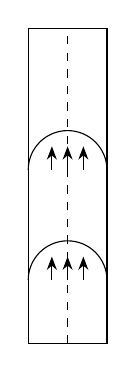
\begin{tikzpicture}[
    >=Stealth,
    3d/.style={z={(0,-0.5cm)}, x={(1cm,0)}, y={(0,1cm)}} % 3D视角设置
]

% ========== 右侧：井内放大示意图 ==========
\begin{scope}[xshift=4cm]
    % 井筒矩形
    \draw (0,0) rectangle (1,4);
    
    % 中间虚线
    \draw[dashed] (0.5,0) -- (0.5,4);

    
    % 下部两个半圆带箭头
    \foreach \y in {0.8, 2.2} {
        \draw (0,\y) arc[start angle=180, end angle=0, radius=0.5]; % 上半圆
        \foreach \x in {0.3,0.5,0.7} {
            \draw[->] (\x,\y) -- (\x,\y+0.3); % 小箭头
        }
    }
\end{scope}

\end{tikzpicture}
\end{document}